
\newcommand{\dpt}[1]{\frac{\partial #1}{\partial t}}
\newcommand\pijk{\phi_{i,j,k}}

\subsubsection{Advection of a generic conserved quantity}

Consider the advection of a generic {\em conserved} quantity $\phi$ by a continuous velocity field
\be
\dert \phi + \nabla \cdot ( \phi \,\U)  = 0. 
\label{phiconv}
\nd
We assume that $\phi$ is smoothly varying except on the interface where it may be discontinuous.
Indeed finding a correct scheme for the advection of this discontinuity, at the same speed as the advection of the 
volume fraction, is the goal of the present study.
The smoothness of the advected quantity away from the interface
is verified for the density $\rho$, the momentum $\rho \U$ or the internal energy 
$\rho e$. We first integrate \eqref{phiconv} in time
\be
{\pijk^{n+1} - \pijk^{n}} = - \sum_{\rm{faces}\, f} F^{(\phi)}_f, \label{sumfp}
\nd
The sum on the right-hand side is the sum over faces $f$ of cell $i,j,k$ 
of the fluxes $F^{(\phi)}_f$ of $\phi$, which are defined as the color function fluxes
$F^{(c)}_f$ in \eqref{faceint}
\be
F_f^{(\phi)} = \int_{t_n}^{t_{n+1}} {\rm d}t \int_{f} u_f(\X,t) \,\phi(\X,t) \,
{\rm d}\X.
\label{pfaceint}
\nd
In order to ``extract'' the discontinuity we introduce the 
 characteristic function $H(\X,t)$
\be
F_f^{(\phi)} = 
\int_{t_n}^{t_{n+1}} {\rm d}t \int_{f} [ u_f  \,H \,\phi  +  u_f \,(1-H) \,\phi ] 
\, {\rm d}\X \,, 
\label{fluxphi}
\nd
and rewrite it as
\be
F_f^{(\phi)} = 
\bar \phi_1 \int_{t_n}^{t_{n+1}} {\rm d}t \int_{f} u_f \,H \,{\rm d}\X + 
\bar \phi_2 \int_{t_n}^{t_{n+1}} {\rm d}t \int_{f} u_f \,(1-H) \,{\rm d}\X \,,
\label{barphi}
\nd
where the face averages $\bar \phi_s$, $s=1,2$, are
\be 
\bar \phi_s = \frac{\int_{t_n}^{t_{n+1}} {\rm d}t \int_{f} \phi \,u_f \,H_s  
{\rm d}\X}{\int_{t_n}^{t_{n+1}} {\rm d}t \int_{f}  
u_f \,H_s\,{\rm d}\X} \,,  
\label{barphi2}
\nd
and $H_1=H$, $H_2= 1-H$. Expression \eqref{barphi} can be written in terms 
of the fluxes $F^{(c)}_f$ and $F^{(1-c)}_f$, this second one being obtained by 
replacing $H$ with $1-H$ in \eqref{faceint}
\be
F_f^{(\phi)} = \bar \phi_1 \,F_f^{(c)} +  \bar \phi_2 \,F_f^{(1-c)} \,.
\label{fluxphi12}
\nd

\subsubsection{Cloning the tracers}

When a cell is cut by the interface, and the field $\phi$ is not smooth, 
it becomes difficult to estimate the integrals in (\ref{barphi}). A possibility is to 
define two new fields $\phi_{1}$ and $\phi_{2}$, with $\phi_s = \phi$ 
inside phase $s$, then
\be
\phi = H \,\phi_1 + (1-H) \,\phi_2 \,.
\nd
This is more costly in memory usage but simplifies considerably the computation of the 
averages in (\ref{barphi}). The two equations \eqref{interfadv} and \eqref{phiconv} 
are now replaced by three equations,
the same volume fraction equation (\ref{interfadv}) and 
\be
\dert \phi_1 + \nabla \cdot ( \phi_1 \U) = 0 \,\,,\qquad
\dert \phi_2 + \nabla \cdot ( \phi_2 \U) = 0 \,.
\label{pcv1}
\nd
% \bea
% \dert \phi_1 + \nabla \cdot ( \phi_1 \U)  &= 0&  \label{pcv1}, \\ 
% \dert \phi_2 + \nabla \cdot ( \phi_2 \U)  &= 0& \label{pcv2} . 
% \nda
The three equations \eqref{interfadv} and \eqref{pcv1} now imply (\ref{phiconv}). 
The addition of a pair of ``cloned'' variables to deal with large 
variations of density is similar to the methods used for the resolution of the 
momentum and energy equations for compressible flow. For example Saurel and Abgrall 
used two density, momentum and energy variables in their seven-equations model 
\cite{Saurel99}, while Allaire, Clerc and Kokh use two density variables 
in their five-equations model \cite{allaire02}. The addition of a cloned 
tracer variable in incompressible isothermal flow was also implemented by Popinet in 
the ``Basilisk'' code \cite{basilisk}. 

\subsubsection{Advection of the density field}

The density $\rho(\X,t)$ obeys (\ref{phiconv}) with $\phi = \rho$. 
Moreover we consider a divergence-free velocity field, with constant density 
in each phase. We can extract the density trivially from the integrals 
\eqref{barphi2} to obtain {\em exactly} $\bar \rho_s = \rho_s$. 
The flux of $\rho$ is then
\be
F_f^{(\rho)} = \rho_1 F_f^{(c)} +  \rho_2 F_f^{(1-c)}.\label{fluxrho}
\nd
Using this flux definition for $\rho$, and any VOF method for the fluxes of the color 
function, one obtains a conservative method for $\rho$, since eq. (\ref{sumfp}) 
evolves $\rho$ as a difference of fluxes. Thus the total mass is conserved. 
However this result is not consistent with the advection of the color function in the 
CIAM case, as CIAM does not conserve volumes exactly (see  \eqref{sumfall}).
As a result the advection of $\rho$ 
is not consistent with the advection of $C$. 

This paradox may be resolved if one notices that the compression term is missing 
in \eqref{phiconv}. For consistency the compression term should be kept,
and the advection equation for a conserved quantity becomes
\be
\dert \phi + \nabla \cdot ( \phi \,\U)  = \phi \, \nabla \cdot \U \label{phiconv2}
\nd
It is then possible to define the evolution of $\phi$ through a sequence of 
directionally split operations which are equivalent to the operations performed on 
the color function 
\be
{\pijk^{n,l+1} - \pijk^{n,l}} = - F^{(\phi)}_{m-} - F^{(\phi)}_{m+} 
+ \Big( \tilde \phi_1^m c^{(1)}_m + \tilde \phi_2^m c^{(2)}_m \Big) \,
\partial_{m}^h u_m \label{sumfpconsistent}
\nd
where $F^{(\phi)}_{m\pm}$ are defined in \eqref{fluxphi12}, 
the cell averages $\tilde \phi_s^m$ are
\be
\tilde \phi_s^m = \frac{\int_{t_n}^{t_{n+1}} {\rm d}t \int_{\Omega}  \phi  H_s  
\partial_{m}^h u_m  \,  {\rm d}\X}
{\int_{t_n}^{t_{n+1}} {\rm d}t \int_{\Omega} H_s  \partial_{m}^h u_m \,{\rm d}\X} \,,
\label{cellphi2}
\nd
and $c^{(1)}_m=c_m$ is the compression coefficient of the VOF advection,
while $c^{(2)}_m= 1 -c_m$ is that of the symmetric color fraction  $1 - C$.
Specifically for $\rho$ this gives 
\newcommand\rijk{\rho_{i,j,k}}\be
{\rijk^{n,l+1} - \rijk^{n,l}} = - F^{(\rho)}_{m-} - F^{(\rho)}_{m+} + C_m^{(\rho)}\,,
\label{sumfrho}
\nd
where the fluxes are given by (\ref{fluxrho}) and the compression term is
\be
C_m^{(\rho)} =  \Big( \rho_1 c^{(1)}_m + \rho_2 c^{(2)}_m \Big) \,\partial_{m}^h u_m  
\label{central}
\nd
with no implicit summation on $m$ and $c_m^{(s)}$ given by (\ref{cmle}) or
(\ref{cmwy}). 
For the WY method, the compression terms eventually cancel and mass is conserved 
at the same accuracy as the discrete incompressibility condition
$\sum_{m=1}^3 \partial_{m}^h u_m=0$ is verified. 

\subsubsection{Momentum advection: basic expressions}

For momentum advection we consider the transport of the scalar quantities  
$\phi=\rho u_q$, where $q=1,2,3$ is the component index. 
With definition (\ref{barphi2}), we obtain for the face weighted averages 
$\bar \phi_s = \overline { \rho u_q}_s$ the expression
\be 
\overline{\rho u_q}_s = \rho_s \bar u_{q,s} 
\nd
where 
\be \bar u_{q,s} =  \frac{\int_{t_n}^{t_{n+1}} {\rm d}t \int_{f}  u_q u_f  H_s  \, {\rm d}\X}{\int_{t_n}^{t_{n+1}} {\rm d}t \int_{f}  u_f  H_s\,{\rm d}\X} \label{barudef}
\nd
We term $\bar u_{q,s}$ the ``advected interpolated velocity'' and 
explain below how it is computed. 
Thus the evolution of the momentum is given by
\newcommand\mijk{(\rho u_{q})_{i,j,k}}
\begin{eqnarray}
{\mijk^{n,l+1} - \mijk^{n,l}}  = - F^{(\rho u)}_{m-} - F^{(\rho u)}_{m+}
 + \Big( \rho_1 \tilde u_{q,1}^m  c^{(1)}_m +  \rho_2 \tilde u_{q,2}^m c^{(2)}_m 
 \Big) \, \partial_{m}^h u_m 
\label{sumfrou}
\end{eqnarray}
% \begin{eqnarray}
% {\mijk^{n,l+1} - \mijk^{n,l}} & = &  \nonumber \\
% - F^{(\rho u)}_{m-} - F^{(\rho u)}_{m+}
%  + ( \rho_1 \tilde u_{q,1}^m  c^{(1)}_m &+ & \rho_2 \tilde u_{q,2}^m c^{(2)}_m ) \partial_{m}^h u_m 
% \label{sumfrou}
% \end{eqnarray}
where
\be
 F^{(\rho u)}_{f} =  \rho_1 \,\bar u_{q,1}  \,F^{(c)}_{f}  +  
 \rho_2 \,\bar u_{q,2}  \,F^{(1-c)}_{f} \,,
\nd
and the ``central interpolated velocity'', corresponding to the 
averages $\tilde \phi_s^m$ of \eqref{cellphi2}, are
\be
\tilde u_{q,s}^{m} = \frac{\int_{t_n}^{t_{n+1}} {\rm d}t \int_{\Omega} u_q \, H_s \,  
\partial_{m}^h u_m   \,  {\rm d}\X}
{\int_{t_n}^{t_{n+1}} {\rm d}t \int_{\Omega} H_s \, \partial_{m}^h u_m \,{\rm d}\X} 
\label{tildeudef}
\nd
From now on we omit the superscript $m$ 
for $\tilde u_q^m$ to avoid too complex notations. 
Notice that ``cloning'' the advected velocities 
$\bar u_{q,1}$ and $\bar u_{q,2}$
would make it easier to advect a velocity field with a jump on the interface. 
However in viscous flow without phase change the velocity is continuous on the 
interface, and to avoid an excessively complicated method we 
approximate the velocity field as continuous and we choose 
$\bar u_q =  \bar u_{q,1} = \bar u_{q,2}$ for the 
``advected interpolated velocity'' and $\tilde u_q =  \tilde u_{q,1} = \tilde u_{q,2}$
for the ``central interpolated  velocity''. An important simplification is then 
\be
 F^{(\rho u)}_{f} = \bar u_q F^{(\rho)}_{f} \label{frou}
\nd
(which is the central equation in this development) and thus
\be
{\mijk^{n,l+1} - \mijk^{n,l}} =  -\bar u_q  F^{(\rho)}_{m-} - \bar u_q  F^{(\rho)}_{m+} 
+ \tilde u_q C_m^{(\rho)},
\label{sumfmom2}
\nd
where the density fluxes are defined in (\ref{fluxrho}) and the compression term 
$C^{(\rho)}$ in (\ref{central}). 
In the above expression the face-weighted average velocities $\bar u_q$ are defined
using (\ref{barudef}) on the corresponding
left face $m-$ or right face $m+$. It is important to note that up to this point
the weighted averages  $\bar u_q$ and $\tilde u_q$ have been defined but the method
in which they are estimated in the numerical method will be given only in what follows.

If we combine the scheme above with the CIAM scheme, the compression coefficient
in the volume fraction advection from \eqref{cmle} is $C^{n,l}$, and for the 
central interpolated velocity we take $\tilde u_q = u_q^{n,l}$. The compression
term in (\ref{sumfmom2}) does not cancel out when the final momentum is computed 
after three directionally-split advections and the result is not exactly conservative. 
On the other hand with the WY scheme, the compression coefficient
in the volume fraction advection from \eqref{cmwy} is $c$,
that is independent of direction $m$ and \eqref{central} becomes
\be
C_m^{(\rho)} =  \Big( \rho_1 c + \rho_2 (1-c ) \Big) \,\partial_{m}^h u_m  \,.
\label{central2}
\nd
Since there is no bracketing on the velocity components, we take 
$\tilde u_q = u_q^{n}$ which is independent on the substep $l$.
Provided the velocity field is incompressible, that is 
$\sum_{m=1}^3 \partial_{m}^h u_m =0$, after the three split advections (\ref{sumfmom2}) 
one obtains a cancellation of the compression terms and 
\be
{\mijk^{n,3} - \mijk^{n}} =  - \sum_{\rm faces \, f}  \bar u_{q}  F^{(\rho)}_{f} . 
\label{sumfmomtotfracstep}
\nd
The momentum transport coupled with WY advection is thus exactly 
conservative. The advected interpolated velocity $\bar u_q$ and the velocity
$u_f$ normal to face $f$ are discussed in the next section.

\subsubsection{Momentum advection: interpolations and flux limiters}

The momentum equation (\ref{sumfmom2}) can be approximated either
 1) in the bulk of the phases or 2) in the neighborhood of the interface.
In the first case the expression simplifies considerably since both the density
and the color fraction are constant and the spurious compression terms cancel out
\be
{u^{n,3}_q - u_q^{n}} =  - \sum_{\rm faces \, f}  \bar u_{q} u_f . \label{sumfmomtot}
\nd
We distinguish an ``advecting'' velocity $u_{f}= \U \cdot \N_f $ and an ``advected velocity'' 
component $\bar u_{q,f}$, involving an average over face $f$. Both velocity components
require an interpolation from their position in the staggered grid to where they are needed.
Thus the scheme in the bulk is 
\be
{u^{n,3}_q - u_q^{n}} =  - \sum_{\rm faces \, f}  \bar u_{q}^{\rm (advected)} 
u^{\rm (advecting)}_f \,,  
\label{sumfmomtotbulk}
\nd
while near the interface is 
\be
{(\rho u_q)^{n,3} - (\rho u_q)^{n}} =  - \sum_{\rm faces \, f}  \bar u_{q}^{\rm (advected)}  
F^{(\rho)}_{f} + \sum_{m=1}^3 \tilde u_q C_m^{(\rho)} \,. 
\label{advect-ed-ing-2}
\nd
Momentum advection in our model is described by these two equations which are
solved on a cubic grid with a finite-volume method. In the previous sections
we have derived a new expression for the momentum fluxes and the
compression term, i.e. the RHS of \eqref{advect-ed-ing-2}, that is consistent
with the volume fraction advection.  

To estimate the advecting velocities $u_f^{\rm (advecting)}$ we use a centered scheme.
The staggered 2D grid of Fig. \ref{stag-grid} has the same variables
arrangement that is found in 3D on a plane perpendicular to the $z$-axis and through the 
pressure point $p_{i,j,k}$. To illustrate the procedure we consider a face perpendicular
to the horizontal direction $1$, in particular $f=1-$. 
There are two cases. In the first case the advected component is not aligned with the 
face normal, this corresponds to $q=2$. The $u_2$ control volume in 
Fig. \ref{stag-grid} is centered on $i,j+1/2,k$, and face $f=1-$ is then 
centered on $i-1/2,j+1/2,k$. The advecting velocity  $u_{1-}^{\rm (advecting)}$ 
is not given on this point and has to be interpolated 
\be
 u_{1;i-1/2,j+1/2,k}^{\rm (advecting)} = \frac12 \big( u_{1;i-1/2,j,k} + u_{1;i-1/2,j+1,k} 
\big) \,.
\label{uf2}
\nd
In the second case the advected component is aligned with the 
face normal, this corresponds to $q=1$. The $u_1$ control volume 
in Fig. \ref{stag-grid} is centered on $i+1/2,j,k$ and face $f=1-$ is then 
centered on $i,j,k$. The interpolation is now
\be
 u_{1;i,j,k}^{\rm (advecting)} = \frac12 \big( u_{1;i-1/2,j,k} + u_{1;i+1/2,j,k} \big) \,.
\label{uf1} 
\nd
 
Now we turn to the interpolation of the {\em advected} velocity $\bar u_{q}$ in
(\ref{advect-ed-ing-2}). The interpolants we use in this case are
one-dimensional and operate on the velocities $u_q$, on the center of their 
control volume, that are regularly spaced on a segment aligned 
with the direction of the advection, that is perpendicular to face $f$. 
We still consider an advection along the horizontal direction $1$. 
In Fig. \ref{advect-ed-ing-fig}, with the lighter notation $\phi = u_q$,
we need to interpolate the advected velocity on the left face
of the reference control volume $\Omega$.
For the advected velocity $u_1$ and the advecting velocity \eqref{uf1} on face
$f=1-$ the correspondence with the $\phi$ values in Fig. \ref{advect-ed-ing-fig} is
\be
\phi_{-3/2} = u_{1;i-3/2,j,k}, \quad \phi_{-1/2} = u_{1;i-1/2,j,k}, \quad   
\phi_{1/2} = u_{1;i+1/2,j,k}, \;\cdots
\nd
while for the advected velocity  $u_2$ and the advecting velocity \eqref{uf2} is
\be
\phi_{-3/2} = u_{2;i-2,j+1/2,k}, \quad  \phi_{-1/2} = u_{2;i-1,j+1/2,k}, 
\quad  \phi_{1/2} = u_{2;i,j+1/2,k}, \;\cdots
\nd
The extension of these results to an advection along the other two directions $q=2,3$ 
follows easily. We need to predict $\phi_0$ on face $f=1-$ in Fig. \ref{advect-ed-ing-fig}
to serve as an approximation of $\bar u_q$ given in (\ref{barudef}). We consider 
an interpolation function $f$ that computes 
this value as a function of the four nearest points,
and in an upwind manner based on the sign of the {\em advecting} velocity $u_f$
\be
\phi_0 = f \big( \phi_{-3/2}, \phi_{-1/2}, \phi_{1/2},\phi_{3/2},{\rm sign}(u_f)
\big) \,.
\label{simpleinterp}
\nd

In this study we have extensively tested two kinds of interpolations:
\begin{enumerate}
\item a scheme that uses a QUICK third order interpolant in the bulk, away from the interface 
and a simple first order upwind flux near the interface. We call this scheme QUICK-UW;
\item a scheme that uses a Superbee slope limiter \cite{roe1985some} for the flux in the 
bulk and a more complex Superbee limiter tuned to a shifted interpolation point near the 
interface.  We naturally call this scheme ``Superbee''. 
\end{enumerate}
The details of the two schemes are given in \ref{appinterp}.
\begin{figure}
\begin{center}
    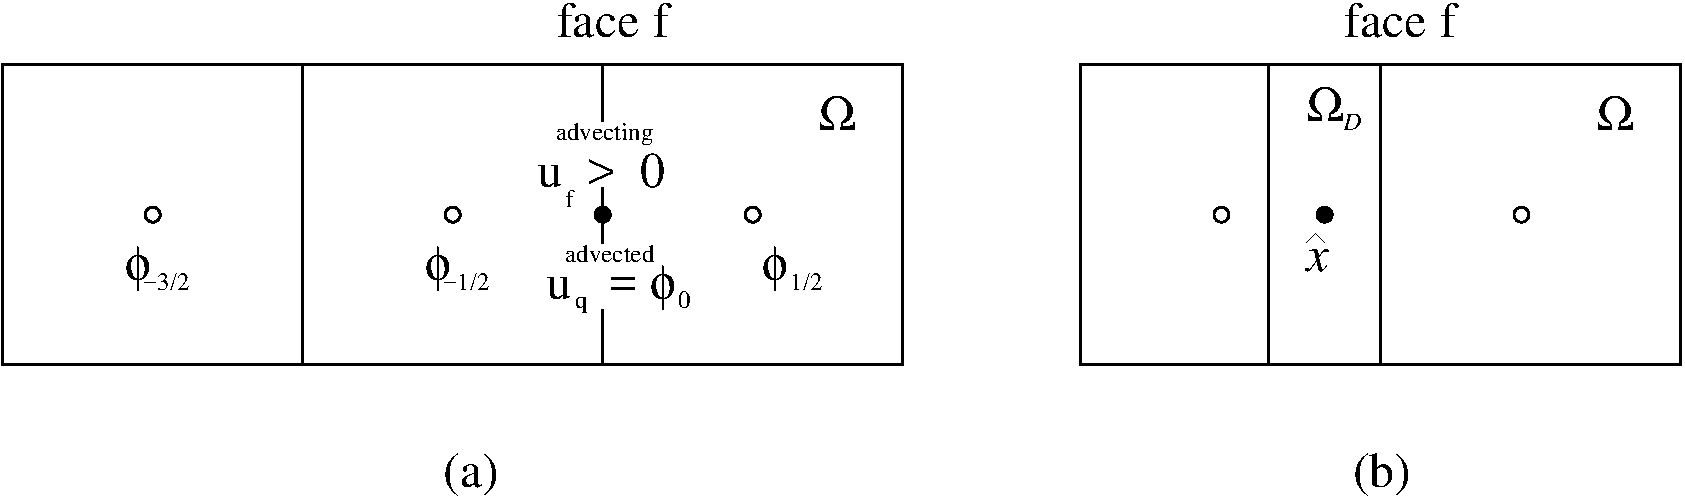
\includegraphics[width=\textwidth]{Figures/advect-ed-ing.pdf}
\end{center}
\caption{The reference control volume $\Omega$ for the advected velocity component 
$\phi=u_q$ is shown. A horizontal advection is here considered and both the advecting velocity 
$u_f$ and the advected velocity require an interpolation for their value on the left face 
$f=1-$: (a) the value $\bar u_q = \phi_0$ (full circle) is interpolated 
(see \ref{appinterp}) from the values $\phi=u_q$ on the nodes (open circles);
(b) a more sophisticated interpolation predicts the value $\phi(\hat x)$ where $\hat x$ is
at the center of the ``donating'' region $\Omega_D$ (see \ref{appinterp}).}
% \caption{(a) The advected and advecting velocities in expression (\ref{advect-ed-ing-2}) 
%   are both located on or near face $f$ (in this case $f=1-$). The reference control volume
% $\Omega$ for the advected velocity component $u_q$ is also shown. The arrangement is the same
% whatever the component $q$ but here the example of a horizontal advection ( case $f=1-$ ) is taken. 
% The value of the advected velocity component $\bar u_q = \phi_0$ on the center of 
% face $f$ (full disk) is interpolated (see text) from the values $\phi_{p}$ of $u_{q}$ on the nodes (open disks). 
% (b) A more sophisticated interpolation predicts the value $\phi(\hat x)$ where $\hat x$ is
% at the center of the ``donating'' region $\Omega_D$ (see text).}
\label{advect-ed-ing-fig}
\end{figure}
%\subsubsection{Momentum advection: tuned interpolations near the interface}
\label{tunedinter}

\subsubsection{VOF-consistent momentum advection on staggered grids}

In order to apply the above method on the staggered grid, we need
the color fraction data in the velocity control volumes. 
At the start of the velocity advection operations, summarized by the operator 
$\LLL^h_{\rm conv}$, each velocity control volume overlaps two pressure/VOF 
control volumes, for example $\Omega_{i+1/2,j}$ overlaps $\Omega_{i,j}$ and $\Omega_{i+1,j}$ 
in the 2D case of Fig. \ref{halffractions}. An estimate of the shifted volume fraction
$C_{i+1/2,j}$ in $\Omega_{i+1/2,j}$ is then obtained by performing the usual reconstructions
in $\Omega_{i,j}$ and $\Omega_{i+1,j}$  and adding the two half-fractions.
The following operations are then performed at each time step and are summarized
in \textbf{Algorithm 1}:

\begin{algorithm}
\caption{Summary of the algorithm for the momentum and VOF time step}
\label{resumealgo}
\begin{algorithmic}[]
   \State Reconstruct interface from volume fractions $C^{n}$
   \For {each component $q$}
      \State Compute ``shifted'' volume fraction $C^{n,0}_q$ in the staggered control volumes 
      \State Compute density $\rho^{n,0}_q$ (Eq. \ref{muH})
      \State Compute momentum component $(\rho_q u_q)^{n,0}$
   \EndFor
   \For {each substep $l$}
      \For {each component $q$}
         \State Momentum advection in the $x_l$ direction to compute $(\rho_q u_q)^{n,l+1}$ 
                (Eq. \ref{sumfmom2})
         \State (the $x_l$ coordinate direction changes with the time step)
         \State VOF advection of ``shifted'' $C_q$ in the $x_l$ direction to compute 
                $C^{n,l+1}_q$
         \State Compute density $\rho^{n,l+1}_q$ (Eq. \ref{muH})
         \State Update velocity component $u_q^{n,l+1} = (\rho_q u_q)^{n,l+1}/\rho^{n,l+1}_q$
      \EndFor
      \State VOF advection of $C$ in pressure control volumes in the $x_l$ direction
             to compute 
      \State $C^{n,l+1}$
   \EndFor
\end{algorithmic}
\end{algorithm}

\begin{enumerate}
\item Reconstruction of the interface at time $t_n$ from the data $C^{n}$,
and computation of the shifted fraction of Fig. \ref{halffractions} to obtain
the ``shifted'' data $C^{n}_q$ and $\rho^{n}_q$ in the staggered control volumes
($q=1,2,3$ is the component index), for example $\rho_1$ in $\Omega_{i+1/2,j,k}$ for the 
horizontal momentum component $\rho_1 u_1$.
\item Computation of the three momentum components $(\rho_q u_q)^{n}$
at time $t_n$.
\item Advection of the three momentum components along one coordinate direction,
say $x$ direction, using \eqref{sumfmom2} to obtain the updated momentum components 
$(\rho_q u_q)^{n,1}$ after the first substep.
\item Advection with the VOF method of the ``shifted'' volume fraction data $C^{n}_q$ 
of the staggered control volumes along the $x$ direction to obtain the updated volume 
fractions $C^{n,1}_q$ and from \eqref{muH} the densities $\rho_q^{n,1}$ after the first 
substep. 
\item Extraction of the provisional velocity components $u_q^{n,1}$
after the first substep, $u_q^{n,1} = (\rho_q u_q)^{n,1}/\rho_q^{n,1}$.
\item Repeat the previous operations for momentum components, shifted
volume fractions and densities, and velocity components for the next two substeps
with split advections along the $y$ and $z$ directions.
Eventually obtain $(\rho_q u_q)^{n+1} = (\rho_q u_q)^{n,3}$ and 
$\tilde \rho_q^{n+1} = \rho_q^{n,3}$. At each time step, the sequence $x, y, z$
is permuted. 
\item In parallel, computation of $C^{n+1} = C^{n,3}$ on the pressure control volumes using
the VOF method. 
\end{enumerate}

\begin{figure}
\begin{center}
    \includegraphics[width=0.5\textwidth]{Figures/halffractions.pdf}
\end{center}
\caption{Computation of the shifted volume fractions from the half-fractions.}
\label{halffractions}
\end{figure}

The interface reconstruction, the computation of volume fraction fluxes and the 
interpolation of ``advected'' and ``advecting'' velocity components have been 
detailed in the previous sections. 
We remark that the advected velocity components $u_q$ are updated at each substep,
while the advecting velocities $u_f$ are interpolated from the initial
velocity field $\U^n$ at time $t_n$. The shifted fractions of Fig. \ref{halffractions}
are computed by the same routine that is computing the Eulerian fluxes $V_1$ and
$V_3$ of Fig. \ref{eulflux}.

The three momentum components $(\rho_q u_q)^{n+1}$ at the beginning of next time step
$t_{n+1}$ require the computation of the three ``shifted''  volume fractions $C^{n+1}_q$
and densities $\rho^{n+1}_q$ starting from $C^{n+1}$. However, these densities
$\rho^{n+1}_q$ are different from the densities $\tilde \rho_q^{n+1} = \rho_q^{n,3}$
computed in the previous  time step by directly advecting the 
``shifted'' volume fractions $C^{n}_q$. The reason for this difference is that the
linear reconstruction is approximate and it is not even continuous on the 
boundary of its control volume. As a matter of facts, at each substep we have
four slightly different interface reconstructions. This implies that momentum is
not conserved between two time steps. We note that  attempting to always use only the three 
sets $C^{n}_{q}$  and evolve them by the VOF method on the staggered cells 
would maintain conservation but result in the three staggered grids evolving independently 
of each other and eventually diverging.
A diagram of the whole scheme is presented in Fig. \ref{figscheme}.
\begin{figure}
\begin{center}
    \includegraphics[width=\textwidth]{Misc/momcons_diagram_revised}
\end{center}
\caption{Diagram of the time step. For simplicity is represented the 2D case for the
density on the grid $i,j$ and horizontal velocity $u_1$ on the staggered grid $i+1/2,j$.
The evolution of the velocity component $u_2$ on the staggered grid $i,j+1/2$ is similar.
The initial variables $\rho^n$, $u_1^n$, $u_2^n$ are inside the ellipses. The interpolated
``advecting'' components $u_1$ and $u_2$ have superscript $n$. The shifted density $\rho^{n,0}$
is constructed with the shifted fractions of $C$ to initialize the momentum component
$(\rho u_1)^{n,0}$. The first split advection is along the $x$ direction  to 
variables with superscript $n,1$, the second one is along the $y$ direction to
variables with superscript $n,2$. The updated density is $\rho^{n,2}=\rho^{n+1}$
while the horizontal velocity $u_1^{n,2}=u_1^{*}$ enters the RHS of the Poisson-like
equation \eqref{Pois}.}
\label{figscheme}
\end{figure}
%\clearpage

\subsection{Description of the other time-split terms}

The other time-split terms in equation (\ref{conspredictedvel}) and in the projection
step (\ref{fotm}) are solved in a standard centered way. The density on the faces
of the central cells $\Omega_{i,j,k}$ is estimated using a simple average
$\rho_{i+1/2,j,k} = (\rho_{i,j,k} + \rho_{i+1,j,k})/2$. Although this is less accurate and 
consistent than the usage of the densities $\rho_d$, computed from
the shifted fractions as described above, the simple average 
is used both for simplicity and because tests have shown that the usage
of $\rho_d$ leads to less stable simulations. 

The velocities in the diffusion term are introduced in an explicit way. Although this requires small
time steps of the order $\rho h^2/\mu$, the capillary restriction on time steps
is usually even smaller, being of order $\tau = (\rho h^3/\sigma)^{1/2}$. The two restrictions
become of the same order when $h \sim l_{\mu \sigma}$, where $l_{\mu \sigma} = \mu^2 / (\sigma \rho)$ 
is the length at which the viscous and capillary terms balance. For water, this length is 
of the order of 10 nanometers, and grids of that size are not used in the flows we consider. 
However, should the velocities be treated in an implicit manner, we do not believe this would
change the conclusions of this paper. 

Surface tension is computed using the Continuous Surface Force method proposed by 
\cite{brackbill92}, together with an estimate of the curvature through the computation
of height functions, in a manner that closely follows the method of \cite{popinet09}. 
The external forces in equation (\ref{conspredictedvel}) 
are only gravity and are computed in a trivial manner with 
$\frac 1 {\rho^{n+1}} \LLL_{ext} =  \G$, where gravity $\G$  is a constant. 


